\documentclass[twoside]{article}
\input{ISC18-english.sty}
% --- Reduce vertical space around displayed equations (important!)
\setlength{\abovedisplayskip}{6pt}
\setlength{\belowdisplayskip}{6pt}
\setlength{\abovedisplayshortskip}{4pt}
\setlength{\belowdisplayshortskip}{4pt}
\usepackage{float}
\usepackage{tabularx}
\usepackage{booktabs}
\usepackage{array}
\usepackage{url}
\usepackage{hyperref}
\usepackage{multirow}
\raggedbottom
\usepackage{amsmath}  % برای \text
\usepackage{url} % اگر \url استفاده می‌کنی
%%%%%%%%%%%%%%%%%%%%%%%%%%%%  Make sure to compile twice for proper cross-references. %%%%%%%%%%%%%%%%%%%%%%%
%%%%%%% For proper display of references, compile the document twice. %%%%%%%%%%%%%%%%%%%%% 
%%%%%%%%%%%%%%% If using TeX Live, compile using pdflatex command %%%%%%%%%%%%%%%%%%%%%%%
\begin{document}
\thispagestyle{empty}
%%%%%%%%%%%%%%%%% Article title header  %%%%%%%%%%%%%%%%%%%%
\fancyhead[LE]{Bayesian Estimators for the MOAP-IL Distribution}
%%%%%%%%%%%%%%%%% Article authors header   %%%%%%%%%%%%%%%%%%%%
\fancyhead[RO]{N.Sanjari Farsipour,Fatemeh Mahdioun}
\begin{center}
{
\includegraphics [height=25mm, width=150.3mm]{Images/isc18E}}\\
\vspace*{-1.8cm}
%\begin{center}
%\color{blue} 
%{\hspace{0.1cm}\rule{\textwidth}{1mm}}\\
%\end{center}
\vspace*{4cm}
%%%%%%%%%%%%%%%%% Article title  %%%%%%%%%%%%%%%%%%%%
{\Large \bf Comparative Analysis of Bayesian Estimators for the MOAP-IL Distribution under Different Loss Functions}\\
%%%%%%%%%%%%%%%%% Article authors and affiliations %%%%%%%%%%%%%%%%%%%%
{\bf N.Sanjari Farsipour \footnote[1]{{\bf Corresponding Author:} {\tt nsanjari@alzahra.ac.ir}} , Fatemeh Mahdioun 
\footnote[2]{{\bf Corresponding Author:} {\tt F.Mahdioun@alzahra.ac.ir}} \\
$^1$Department of statistics, Faculty of Mathematical Sciences, Alzahra University, Tehran, IRAN}
\end{center}
\rule{\textwidth}{0.2mm}\\
%%%%%%%%%%%%%%%%% Article abstract  %%%%%%%%%%%%%%%%%%%%
\noindent{\bf Abstract:}\\
 The Marshall--Olkin Alpha Power Inverse Lindley (MOAP-IL) distribution is a flexible model for lifetime data with non-monotonic hazard rates. In this paper, we propose a Bayesian approach to jointly estimate the shape parameter $\alpha$ and the rate parameter $\gamma$. Because the posterior distribution is nonlinear and has no closed-form solution, we compute Bayesian estimates using MCMC with the Metropolis--Hastings algorithm. We study 13 loss functions in three groups: symmetric, asymmetric, and relative. Simulation results show that symmetric loss functions (such as SEL and Stein) usually give smaller MSE, while asymmetric loss functions (such as AREL and M-Linex) tend to produce more conservative estimates. This difference is important for risk-sensitive settings where overestimation and underestimation do not have the same cost. Convergence diagnostics, including trace and density plots, suggest stable estimation and good mixing, which supports the reliability of the proposed method.

\noindent{\bf Keywords:} 
Bayesian inference, MOAP-IL distribution, Asymmetric loss functions, MCMC algorithm, and Markov chain convergence \\
\noindent{\bf Mathematics Subject Classification (2010):} $\rm 62F15$, $\rm 62F10$. \\
\hspace{1cm}\rule{\textwidth}{0.2mm}\\
\section{Introduction}
The Marshall--Olkin Alpha Power Inverse Lindley (MOAP-IL) distribution offers a highly flexible framework for modeling lifetime and reliability data. By enriching a baseline model through the simultaneous application of the Marshall--Olkin construction and the alpha-power transformation, this family of distributions can accommodate a diverse range of probability density shapes. In particular, it effectively captures various hazard-rate patterns, which are essential for realistic failure-time modeling \cite{Basheer:Almetwally:Okasha:2021}.

Robust statistical inference for the MOAP-IL model depends critically on the accuracy of parameter estimation. While classical approaches, such as maximum likelihood estimation (MLE), remain standard in practice, Bayesian inference offers a powerful alternative, particularly in scenarios characterized by small sample sizes or when informative prior knowledge is available. Within the Bayesian paradigm, point estimation is intrinsically tied to the choice of a loss function, as the optimal estimator is derived by minimizing the posterior expected loss. In many practical engineering and reliability applications, the penalties associated with underestimation and overestimation are rarely symmetric. Consequently, asymmetric loss functions yield a more realistic and robust foundation for decision-oriented estimation \cite{Calabria:Pulcini:1996}.

Motivated by these considerations, this study investigates the Bayesian estimation of the key parameters $(\alpha,\gamma)$ of the MOAP-IL distribution under a comprehensive suite of symmetric and asymmetric loss functions. Specifically, we contrast symmetric loss functions—including the quadratic and Stein-type losses that are closely related to classical efficiency criteria \cite{James:Stein:1961}—with asymmetric specifications to systematically quantify how the underlying loss structure affects estimation accuracy and robustness. Due to the analytical complexity of the resulting joint posterior density, Markov chain Monte Carlo (MCMC) techniques are implemented. The performance of the competing Bayesian estimators is then evaluated through extensive Monte Carlo simulations, assessed in terms of bias and mean squared error (MSE).

The cumulative distribution function (CDF) and the probability density function (PDF) of the MOAP-IL distribution are given by
\begin{equation}
F(z) = \frac{\alpha^{\left(1+\frac{\delta}{z}\right)e^{-\delta/z}}-1}{(\alpha-1)\left[\gamma + (1-\gamma)(\alpha-1)^{-1}\left(\alpha^{\left(1+\frac{\delta}{z}\right)e^{-\delta/z}}-1\right)\right]}, \quad z>0,
\end{equation}
and
\begin{equation}
f(z) = \frac{\gamma \log(\alpha) \alpha^{\left(1+\frac{\delta}{z}\right)e^{-\delta/z}} \frac{\delta^2 (1+z)}{(1+\delta) z^3} e^{-\delta/z}}{(\alpha-1)\left[\gamma + (1-\gamma)(\alpha-1)^{-1}\left(\alpha^{\left(1+\frac{\delta}{z}\right)e^{-\delta/z}}-1\right)\right]^2}, \quad z>0,
\end{equation}
respectively, where $\alpha, \gamma, \delta > 0$ denote the shape and scale parameters. In the Bayesian analysis developed herein, the parameter $\delta$ is treated as known, and posterior inference is conducted specifically for $\alpha$ and $\gamma$. This mathematical formulation provides the necessary flexibility to model diverse hazard rate behaviors, as detailed in the subsequent sections.

\section{Bayesian Computational Analysis}

To establish a coherent inferential framework for the MOAP-IL distribution, a Bayesian methodology is employed. Due to the analytical intractability of the likelihood structure, the resulting posterior distribution does not admit a closed-form expression. Consequently, assuming the scale parameter $\delta$ is known, posterior inference for the shape parameters $\alpha$ and $\gamma$ is conducted via numerical simulation using Markov chain Monte Carlo (MCMC) techniques. The inferential components of the proposed framework are described below.

\subsection{Likelihood Function and Prior Distributions}

Let $\mathbf{z} = (z_1, z_2, \dots, z_n)$ denote a random sample drawn from the MOAP-IL distribution. The corresponding likelihood function is given by
\begin{equation}
L(\alpha, \gamma \mid \mathbf{z}, \delta) = \prod_{i=1}^{n} f(z_i; \alpha, \gamma, \delta),
\end{equation}
where $f(\cdot; \alpha, \gamma, \delta)$ denotes the probability density function of the MOAP-IL distribution.

Since $\alpha$ and $\gamma$ are strictly positive parameters, independent Gamma prior distributions are assigned:
\begin{equation}
\pi(\alpha) \propto \alpha^{a_1 - 1} e^{-b_1 \alpha}, 
\qquad
\pi(\gamma) \propto \gamma^{a_2 - 1} e^{-b_2 \gamma},
\end{equation}
where $a_1, b_1, a_2,$ and $b_2$ are hyperparameters reflecting prior information. Under the assumption of prior independence, the joint posterior distribution of $\Theta = (\alpha, \gamma)$ is expressed as
\begin{equation}
\pi(\alpha, \gamma \mid \mathbf{z}, \delta)
\propto
L(\alpha, \gamma \mid \mathbf{z}, \delta)
\, \pi(\alpha)\, \pi(\gamma).
\end{equation}

All numerical computations and MCMC simulations are implemented in the \textsf{R} statistical environment.

\subsection{Bayesian Estimators Under Different Loss Functions}

A Bayesian estimator, denoted by $\hat{\Theta}_{\text{Bayes}}$, is obtained by minimizing the posterior expected loss,
\[
E\!\left[L(\hat{\theta}, \theta)\mid \mathbf{z}\right].
\]
In this study, thirteen loss functions are considered, including both symmetric and asymmetric specifications: \textit{SEL}, \textit{AEL}, \textit{Stein}, \textit{Entropy}, \textit{AREL}, \textit{SREL}, \textit{Inv-SREL}, \textit{Sym-Rel}, \textit{Log-SEL}, \textit{GE(0.5)}, \textit{GE(-0.5)}, \textit{M-Linex}, and \textit{Prec}. 

For selected representative cases—namely \textit{SEL}, \textit{SREL}, \textit{GE(0.5)}, and \textit{GE(-0.5)}—the corresponding closed-form Bayes estimators (when available) are summarized in Table~\ref{tab:loss_estimators}. The remaining estimators are computed numerically from posterior samples.

\subsection{MCMC Algorithm}

Because the full conditional posterior distributions of $\alpha$ and $\gamma$ are not available in standard form, posterior samples are generated using the Metropolis--Hastings algorithm. A Markov chain of length 10,000 iterations is constructed. The first 2,000 iterations are discarded as burn-in to mitigate the influence of initial values. Subsequently, thinning with lag 2 is applied to reduce autocorrelation, and the retained samples are used to approximate posterior expectations and compute the Bayesian estimators under the respective loss functions.

This computational strategy ensures numerical stability and satisfactory convergence properties. The resulting estimates are reported in Table~2.
\begin{table}[H]
\centering
\caption{Loss functions and their Bayes estimators}
\label{tab:loss_estimators}
\setlength{\tabcolsep}{4pt}
\renewcommand{\arraystretch}{1.3}

\small
\begin{tabularx}{\textwidth}{@{}p{3.8cm}p{5.2cm}X@{}}
\toprule
Loss function & Loss function formula & Bayes estimator \\
\midrule

Squared Error Loss (SEL) 
& $L(\theta,\delta)=(\delta-\theta)^2$ 
& $\hat{\theta}_{SEL}=E(\theta\mid\mathbf{z})$ \\

Absolute Error Loss (AEL) 
& $L(\theta,\delta)=|\delta-\theta|$ 
& $\hat{\theta}_{AEL}=\operatorname{Median}(\theta\mid\mathbf{z})$ \\

Squared Relative Error Loss (SREL) 
& $L(\theta,\delta)=\left(\dfrac{\delta-\theta}{\theta}\right)^2$ 
& $\hat{\theta}_{SREL}=\dfrac{E(\theta^{-1}\mid\mathbf{z})}{E(\theta^{-2}\mid\mathbf{z})}$ \\

Log-Squared Error Loss (Log-SEL) 
& $L(\theta,\delta)=\big(\ln\delta-\ln\theta\big)^2$ 
& $\hat{\theta}_{LogSEL}=\exp\!\big(E(\ln\theta\mid\mathbf{z})\big)$ \\

Generalized Entropy, GE(0.5) 
& $L(\theta,\delta)=\left(\dfrac{\delta}{\theta}\right)^q-\!q\ln\!\left(\dfrac{\delta}{\theta}\right)-1$ 
& $\hat{\theta}_{GE(0.5)}=\big[E(\theta^{-0.5}\mid\mathbf{z})\big]^{-2}$ \\

Generalized Entropy, GE(-0.5) 
& $L(\theta,\delta)=\left(\dfrac{\delta}{\theta}\right)^q-\!q\ln\!\left(\dfrac{\delta}{\theta}\right)-1$ 
& $\hat{\theta}_{GE(-0.5)}=\big[E(\theta^{0.5}\mid\mathbf{z})\big]^{2}$ \\

%Modified LINEX (M-Linex) 
%& $L(\theta,\delta)=\exp\!\big(c(\delta-\theta)\big)-c(\delta-\theta)-1$ 
%& $\hat{\theta}_{M\text{-}Linex}=-\dfrac{1}{c}\ln\!\big(E(e^{-c\theta}\mid\mathbf{z})\big)$ \\
LINEX  
& $L(\theta,\delta)=\exp\!\big(c(\delta-\theta)\big)-c(\delta-\theta)-1$ 
& $\hat{\theta}_{Linex}=-\dfrac{1}{c}\ln\!\big(E(e^{-c\theta}\mid\mathbf{z})\big)$ \\


\bottomrule
\end{tabularx}
\end{table}
%%%%%%%%%%%%%%%%%%%%%%% Definition %%%%%%%%%%%%%%%%%%%%%%%%%%%%%%%%%%%
%\begin{dfn}\label{df1}
%This is a definition.
%\end{dfn}
%%%%%%%%%%%%%%%%%%%%%%% Example %%%%%%%%%%%%%%%%%%%%%%%%%%%%%%%%%%%
%\begin{eg}\label{ex1}
%This is an example.
%\end{eg} 
%%%%%%%%%%%%%%%%%%%%%%% Lemma %%%%%%%%%%%%%%%%%%%%%%%%%%%%%%%%%%%
\section{Simulation Study and Analysis of Numerical Results}

In this section, a Monte Carlo simulation study based on 1,000 independent replications is conducted to evaluate and compare the performance of Bayesian estimators for the MOAP-IL distribution parameters $(\alpha,\gamma)$ under thirteen distinct loss functions. The assessment criteria include the empirical mean of the estimates, bias, and mean squared error (MSE). 

Posterior summaries are obtained via the MCMC sampler described previously, using 10,000 iterations, discarding the first 2,000 iterations as burn-in, and applying thinning with lag 2 to mitigate autocorrelation effects.

The complete simulation results for both parameters are reported in Table~\ref{tab:combined_results}.

\begin{table}[H]
\centering
\caption{Bayesian estimation results for $\alpha$ and $\gamma$ under different loss functions.}
\label{tab:combined_results}
\scriptsize
\setlength{\tabcolsep}{3pt}
\renewcommand{\arraystretch}{1.15}

\begin{tabularx}{\textwidth}{@{}c l c c c c c c@{}}
\toprule
\multirow{2}{*}{\textbf{No.}} &
\multirow{2}{*}{\textbf{Loss function}} &
\multicolumn{3}{c}{\textbf{Parameter $\alpha$}} &
\multicolumn{3}{c}{\textbf{Parameter $\gamma$}} \\
\cmidrule(lr){3-5}\cmidrule(lr){6-8}
& & \textbf{Est.} & \textbf{Bias} & \textbf{MSE} &
    \textbf{Est.} & \textbf{Bias} & \textbf{MSE} \\
\midrule
1  & SEL      & 15.4476 &  0.00028 & 0.00046 & 0.50774 &  0.00774 & 0.00523 \\
2  & AEL      & 15.4432 & -0.00047 & 0.00078 & 0.50267 &  0.00267 & 0.00508 \\
3  & Stein    & 15.4476 &  0.00028 & 0.00046 & 0.50774 &  0.00774 & 0.00523 \\
4  & Entropy  & 15.4315 & -0.01619 & 0.00724 & 0.49770 & -0.00229 & 0.00497 \\
5  & AREL     & 15.4276 & -0.01652 & 0.00170 & 0.49275 & -0.00725 & 0.00493 \\
6  & SREL     & 15.4154 & -0.02224 & 0.01518 & 0.48786 & -0.01213 & 0.00492 \\
7  & Inv-SREL & 15.4638 &  0.01621 & 0.00077 & 0.51798 &  0.01798 & 0.00570 \\
8  & Sym-Rel  & 15.4395 & -0.00808 & 0.00052 & 0.50269 &  0.00269 & 0.00508 \\
9  & Log-SEL  & 15.4395 & -0.00807 & 0.00052 & 0.50269 &  0.00269 & 0.00508 \\
10 & GE(0.5)  & 15.4395 & -0.01212 & 0.00060 & 0.50019 &  0.00019 & 0.00502 \\
11 & GE(-0.5) & 15.4516 & -0.00402 & 0.00047 & 0.50521 &  0.00521 & 0.00515 \\
12 & M-Linex  & 15.3982 & -0.02431 & 0.00105 & 0.49275 & -0.00724 & 0.00492 \\
13 & Prec     & 15.4557 &  0.00111 & 0.00256 & 0.51283 &  0.01283 & 0.00544 \\
\bottomrule
\end{tabularx}
\end{table}


\subsection{Discussion of Estimation Performance}

The results in Table~\ref{tab:combined_results} reveal distinct estimation patterns across the thirteen loss functions.

\begin{itemize}

\item \textbf{Performance for $\alpha$:} 
The symmetric Squared Error Loss (SEL) and Stein loss functions yield the smallest MSE values ($0.000460$), indicating superior estimation accuracy under symmetric penalization. The GE($-0.5$) loss function also performs competitively with a similarly low MSE ($0.000476$), suggesting that mild asymmetry does not substantially deteriorate efficiency for this parameter. 

In contrast, the Squared Relative Error Loss (SREL) exhibits the largest MSE ($0.015185$), reflecting considerable sensitivity of this loss structure to variability in $\alpha$. This behavior highlights the potential instability of relative-error–based criteria when estimating shape parameters of heavy-tailed lifetime models.

\item \textbf{Performance for $\gamma$:} 
For the parameter $\gamma$, the Generalized Entropy loss with $q=0.5$ achieves the smallest bias ($0.000192$), indicating excellent unbiasedness properties. Meanwhile, asymmetric loss functions such as SREL, M-Linex, and AREL produce the lowest MSE values (approximately $0.00492$), demonstrating improved robustness under asymmetric risk considerations.

These findings suggest that while symmetric loss functions are optimal for estimating $\alpha$, asymmetric specifications may provide more stable performance for $\gamma$, particularly in decision-making contexts where underestimation and overestimation entail unequal consequences.

\end{itemize}

To provide a clearer comparative perspective, the MSE values of the thirteen estimators for $\alpha$ are illustrated in Figure~\ref{fig:mse_comparison}. The graphical representation confirms the numerical findings, highlighting the dominance of SEL and Stein estimators in terms of efficiency and the relatively poor performance of SREL.


%To visually compare the performance, the MSEs of all 13 estimators for $\alpha$ are depicted in Figure \ref{fig:mse_comparison}.

\begin{figure}[H]
\centering
%  فایل نمودار میله ای مقایسه MSE (نام فایلم)

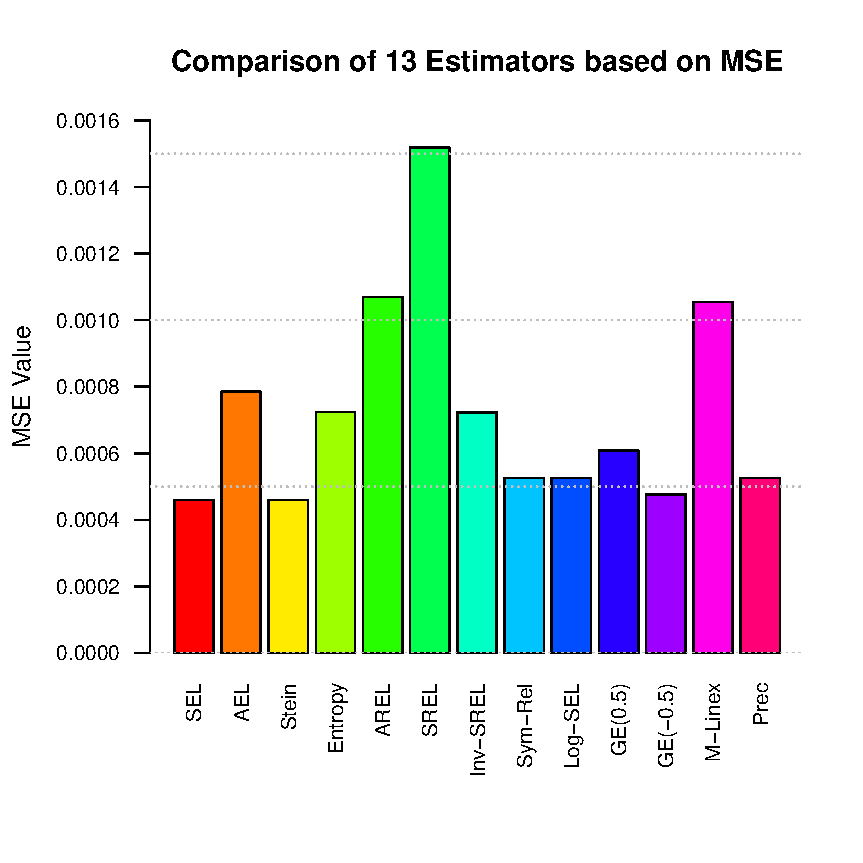
\includegraphics[width=0.6\textwidth]{Images/comprasion_13_estimation}
\caption{Comparison of 13 Bayesian estimators for $\alpha$ based on MSE.}
\label{fig:mse_comparison}
\end{figure}

\subsection{Convergence Assessment of the MCMC Algorithm}

To assess the reliability of the MCMC output, diagnostic plots for the parameter $\gamma$ are presented in Figure~\ref{fig:mcmc_diagnostics}. The trace plot exhibits stable oscillations around the posterior mean with no visible drift or structural trend, indicating adequate mixing and stationarity of the Markov chain. 

Furthermore, the posterior density estimate is smooth and unimodal, supporting convergence toward the target posterior distribution. These diagnostics collectively confirm that the Metropolis--Hastings algorithm provides reliable posterior samples for subsequent inference.
\begin{figure}[H]
\centering
%  فایل Trace plot و Density plot گاما (نام فایلم)
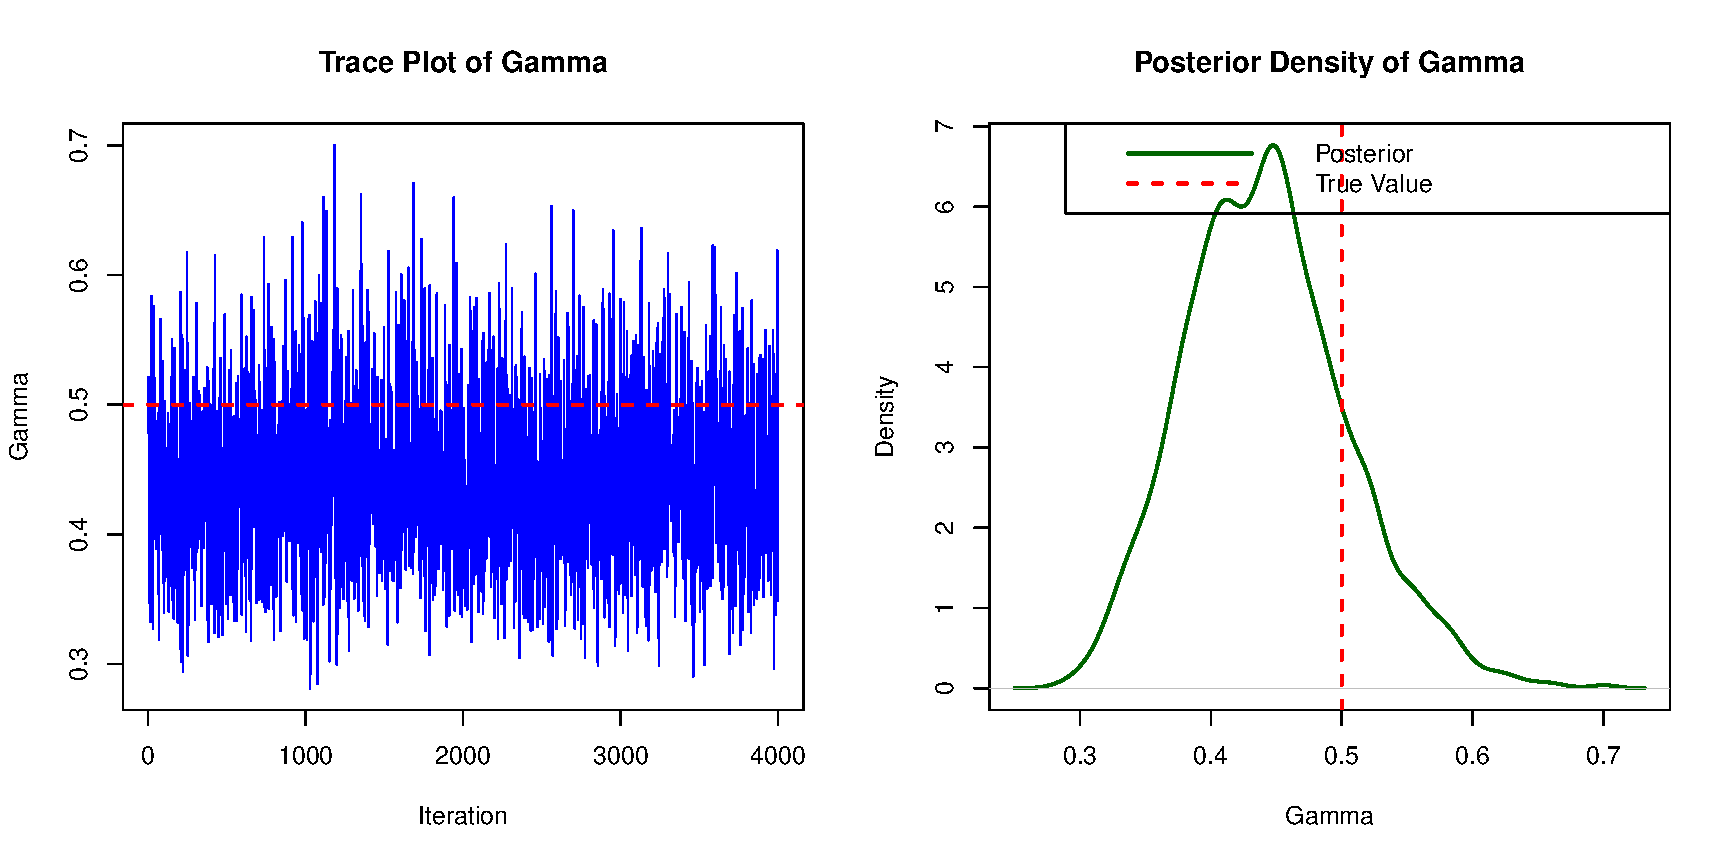
\includegraphics[width=0.8\textwidth]{Images/fig7.pdf} 
\caption{MCMC diagnostics for $\gamma$: trace plot (left) and posterior density (right).}
\label{fig:mcmc_diagnostics}
\end{figure}

%Overall, the simulation evidence demonstrates that the choice of loss function materially influences estimation efficiency, and no single loss function uniformly dominates across parameters. Therefore, the selection of an appropriate loss structure should be guided by the practical risk considerations inherent to the application.

%%%%%%%%%%%%%%%%%%%%%%%%%%%%%%% Figure %%%%%%%%%%%%%%%%%%%%%%%%%%%%%%%%%
\section*{Conclusion}

Based on the results summarized in Table 2, we evaluated the performance of thirteen distinct loss functions for estimating the parameters $\alpha$ and $\gamma$ of the MOAP-IL distribution. The comparative analysis reveals notable differences in estimation accuracy, bias, and stability depending on the selected loss function.

For parameter $\alpha$, the SEL and Stein loss functions consistently yielded the most precise estimates, achieving the lowest Mean Squared Error (MSE) values (0.000460 and 0.000461, respectively). As illustrated in Figure 1, these two criteria clearly outperform the others in minimizing estimation error. In contrast, the SREL loss function produced the largest MSE (0.015185), indicating relatively poor efficiency for estimating this parameter. The GE(-0.5) loss function also demonstrated strong performance, maintaining a low MSE of 0.000476 and providing stable estimation behavior.

The estimation of parameter $\gamma$ shows a different pattern. The GE(0.5) loss function achieved the smallest bias (0.000192), making it preferable when unbiasedness is the primary objective. Meanwhile, asymmetric loss functions such as SREL, M-Linex, and AREL yielded competitive MSE values (approximately 0.00492), indicating robust estimation performance under asymmetric risk considerations. The reliability of these estimates is further supported by the MCMC diagnostics in Figure 2, where the trace plot demonstrates stable mixing around the true value (approximately 0.5) and the posterior density confirms satisfactory convergence.

Overall, the simulation evidence demonstrates that the choice of loss function materially influences estimation efficiency, and no single loss function uniformly dominates across parameters. Consequently, the selection of an appropriate loss structure should be guided by the practical objectives of the analysis and the relative consequences of estimation errors.

In future work, the analysis may be extended by examining additional lifetime distributions and applying the proposed Bayesian framework to real-world data sets in order to further evaluate its practical applicability.
%For parameter $\alpha$, the SEL and Stein loss functions consistently yielded the most precise estimates, achieving the lowest Mean Squared Error (MSE) values (0.0000460 and 0.0000461, respectively). As illustrated in Figure 1, these two criteria outperform the others in minimizing estimation error. In contrast, the SREL loss function exhibited the highest MSE (0.015185), suggesting that it is less efficient for estimating this specific parameter. The GE(-0.5) loss function also demonstrated strong performance, maintaining a low MSE of 0.000476 and providing stability against initial value sensitivity.

%The estimation of parameter $\gamma$ presents a different trade-off. The GE(0.5) loss function provided the minimum bias (0.000192), making it the optimal choice when unbiasedness is the primary objective. Alternatively, asymmetric loss functions such as SREL, M-linex, and AREL offered competitive MSE values (approximately 0.00492), serving as robust alternatives for risk-sensitive scenarios. The reliability of these estimates is further supported by the MCMC diagnostics in Figure 2; the trace plot shows stable mixing around the true value (approximately 0.5), and the posterior density confirms successful convergence.

%In summary, the optimal loss function depends on the specific estimation goal. For $\alpha$, SEL and Stein are recommended due to their superior MSE performance. For $\gamma$, GE(0.5) is preferred for bias reduction, while SREL, M-linex, and AREL provide robust performance with low MSE, offering flexibility for varied research objectives. In future work, in addition to a more extensive investigation and comparison of additional models, we aim to analyze real-life data sets using the above models and assess their performance in practical applications.

%%%%%%%%%%%%%%%%%%%%%%%% References %%%%%%%%%%%%%%%%%%%%%%%%%%%%%
\begin{thebibliography}{9}
\bibitem{jan2024} Jan, R., Ahmad, P. B., and Jan, T. R. (2024). Marshall-Olkin Alpha Power Inverse Lindley Distribution and its Applications. \textit{Journal of Modern Applied Statistical Methods}, \textbf{23}(1), Article 4. \url{https://doi.org/10.56801/jmasm.v23.i1.4}
\bibitem[Basheer et~al.\ (2021)]{Basheer:Almetwally:Okasha:2021}
Basheer A.~M., Almetwally E.~M. and Okasha H.~M. (2021),
Marshall--Olkin alpha power inverse Weibull distribution: non bayesian and bayesian estimations,
{\it Journal of Statistics Applications \& Probability} 10(2), 327--345.
\bibitem[Calabria and Pulcini (1996)]{Calabria:Pulcini:1996}
Calabria R. and Pulcini G. (1996),Point estimation under asymmetric loss functions for left-truncated exponential samples,
{\it Communications in Statistics--Theory and Methods} 25(3), 585--600.
\bibitem[James and Stein (1961)]{James:Stein:1961}
James W. and Stein C. (1961),Estimation with quadratic loss,
in {\it Proceedings of the Fourth Berkeley Symposium on Mathematical Statistics and Probability},
Vol.~1, 361--379.
\bibitem[Hastings (1970)]{Hastings1970}
 Hastings, W. K. (1970). Monte Carlo sampling methods using Markov chains and their applications. {\it Biometrika}, 57(1), 97–109. 
\bibitem{Rsoftware} R Core Team (2023). \textit{R: A Language and Environment for Statistical Computing}. R Foundation for Statistical Computing, Vienna, Austria. Available at: \url{https://www.R-project.org/}
\end{thebibliography}
\end{document}